\documentclass[12pt,letterpaper]{article}
\usepackage[T1]{fontenc}
\usepackage[letterpaper,margin=1in]{geometry}
\usepackage{amsmath,amssymb,amsthm,mathrsfs}
\usepackage{newtxtext,newtxmath}
\usepackage{microtype,booktabs,enumitem,tikz}
\usepackage[hidelinks]{hyperref}
\numberwithin{equation}{section}
\newtheorem{theorem}{Theorem}[section]
\newtheorem{lemma}[theorem]{Lemma}
\newtheorem{proposition}[theorem]{Proposition}
\newtheorem{corollary}[theorem]{Corollary}
\theoremstyle{remark}
\newtheorem{remark}[theorem]{Remark}
\newcommand{\OO}{\mathcal O_F}
\newcommand{\kk}{\mathbb F_q}
\newcommand{\Mp}{\widetilde G}
\newcommand{\cInd}{\operatorname{c-Ind}}
\newcommand{\tr}{\operatorname{tr}}
\newcommand{\val}{\operatorname{val}}
\newcommand{\BT}{\mathscr B}
\title{Notes on characters of supercuspidal representations of the twofold metaplectic cover of $\mathrm{SL}_2(F)$, $F$ $p$-adic\\[.5ex]\large Draft 1: Corrected and expanded version\\A geometric perspective}
\author{David Joyner\thanks{Based on the author's 1996 notes of conversations with Jeff Adams and Jason Schultz. This geometric revisit is a companion to the odd-degree study \cite{Jo26}. Email: \texttt{wdjoyner@gmail.com}.}}
\date{Original draft: 1996. Corrected and expanded draft: 2026\\November 25, 2026}
\begin{document}
\maketitle
\begin{abstract}
This AI-aided paper used Sol-ChatGPT to revise and correct notes written in 1996; see the Acknowledgments for details. We revisit the comparison of characters of ordinary and genuine supercuspidal representations of the twofold metaplectic cover of $\mathrm{SL}_2(F)$ for a $p$-adic field of odd residue characteristic. The Frobenius sums in the original notes are interpreted as weighted sums over fixed vertices in the Bruhat--Tits tree. The two canonical compact splittings have a nontrivial discrepancy on their common Iwahori subgroup, given by a quadratic residue character. This yields a corrected comparison on regular elliptic elements and explicit formulas for generic depth-zero supercuspidals on unramified elliptic tori. The central sign depends on the parity of the vertex orbit and on the residue cardinality modulo four. We also formulate a comparison for arbitrary admissible compact inductions on regular elliptic elements, and identify the additional work required on the split torus and for the full positive-depth classification.
\end{abstract}
\noindent\textbf{2020 MSC:} 22E50, 22E35, 20G05.\\
\textbf{Keywords:} metaplectic double cover, Hilbert symbol, Bruhat--Tits tree, compact induction, character relations.
\tableofcontents

\section{Introduction}\label{sec:intro}
The character of a representation induced from a compact open subgroup is a sum of traces associated with conjugates of that subgroup. The original notes pursued a term-by-term comparison of this sum for linear and metaplectic representations. We preserve this approach, but interpret the conjugates as vertices of a tree. The main issue is no longer whether an individual cocycle expression can be simplified. It is whether the splittings at different fixed vertices agree on the element being studied.

Throughout, $F$ is a finite extension of $\mathbb Q_p$ with $p$ odd. Its ring of integers is $\OO$, its uniformizer is $\varpi$, and its residue field is $\kk$ of order $q$. Write $G=\mathrm{SL}_2(F)$ and let $P:\Mp\to G$ denote the Kubota double cover. A genuine representation is one in which the nonidentity element of $\ker P=\{\pm1\}$ acts by minus the identity. We use the canonical compact splittings $s_v$ over vertex stabilizers $K_v$.

\subsection{Main results and their significance}
The following results distinguish geometric comparison from arithmetic signs. Proposition~\ref{prop:edge} identifies the discrepancy of the splittings on adjacent vertices. It is the quadratic residue character of a diagonal entry of the Iwahori reduction. Theorem~\ref{thm:weighted} expresses the genuine character as an ordinary fixed-vertex trace sum with this discrepancy as a weight. In particular, for regular elliptic elements with reduction having repeated eigenvalue $z=\pm1$, Corollary~\ref{cor:compare} gives a uniform factor
\[
 \Theta_{\widetilde\pi_j}(s_i(t))
 =\ell(z)^{j-i}\Theta_{\pi_j}(t),
\]
where $\ell$ is the quadratic character of $\kk^\times$ and $i,j$ denote vertex types. Thus the comparison holds without a sign on the inducing vertex type, but a sign can appear on the other type.

Theorem~\ref{thm:depthzero} evaluates these sums for generic depth-zero representations. At congruence depth $r\ge1$, the ordinary value is $\theta(z)((-1)^{r+1+j-i}q^r-1)$, and the genuine value is obtained by multiplying by $\ell(z)^{j-i}$. The geometry explains the cancellation of the terms of size $q^r$ in the ordinary packet sum. For the genuine sum, cancellation at $-I$ depends on whether $-1$ is a square in $\kk$. We give a twisted sum that always cancels.

For example, take $F=\mathbb Q_7$. The quadratic character of $-1$ is $-1$. At depth one near $-I$, an ordinary representation induced from the opposite vertex type has character $-8\theta(-1)$, but its genuine counterpart has character $8\theta(-1)$ at the canonical lift from the torus vertex. This sign is invisible in the odd-degree case.

\subsection{Literature review}
The literature supplies the compact constructions and the character-theoretic setting. We separate results available in 1996 from later developments.

\subsubsection{Through 1996}
Kubota \cite{Ku67} constructs the cover using the quadratic Hilbert symbol and gives its splitting over $\mathrm{SL}_2(\OO)$ in odd residue characteristic. Gelbart \cite{Ge76} explains the Weil representation and metaplectic groups. Neukirch \cite{Ne86} supplies the local class field theory behind the Hilbert symbol. For example, the symbol of a uniformizer and a unit detects whether the residue of the unit is a square.

Sally and Shalika \cite{SS68} compute discrete-series characters of $\mathrm{SL}_2(F)$. Deligne and Lusztig \cite{DL76} construct finite reductive-group representations from torus characters. Kutzko \cite{Ku87} develops supercuspidal character sums for $\mathrm{GL}_{\ell}$, with $\ell$ prime. The 1996 notes use a related double-coset organization. We do not invoke a convergence theorem for the cover by analogy alone. On the regular elliptic domain used here, the sum is locally finite for geometric reasons.

Manderscheid \cite{Ma84a,Ma84b} studies supercuspidals of $\mathrm{SL}_2$ and its double cover. The original notes refer to his strongly cuspidal types of level $m>1$ and cuspidal types of conductor one. Moy and Prasad \cite{MP94} place depth-zero constructions in a general building-theoretic framework. Waldspurger \cite{Wa91} develops the theta correspondence, a different kind of comparison from the direct compact-induction relation studied here.

\subsubsection{After 1996}
Joyner \cite{Jo99} treats a metaplectic supercuspidal correspondence in the odd-degree setting. Howard and Weissman \cite{HW09} extend depth-zero theory to tame nonlinear covers, including the metaplectic group in odd residue characteristic. Li \cite{Li12} develops local harmonic analysis for covering groups. Manderscheid \cite{Ma04} studies Waldspurger's involution through types. The companion manuscript \cite{Jo26} gives explicit odd-degree character relations using the two vertex orbits and fixed balls. Its power-map argument uses coprimality of the covering degree with $q+1$, which fails in degree two.

For example, the finite nonsplit torus over $\mathbb F_7$ has order eight. Cubing permutes it, but squaring does not. This paper consequently studies the direct comparison, not a purported inverse-square reparameterization.

\subsection{Notation}
The following notation is used throughout. In the running example $\OO=\mathbb Z_7$ and $\varpi=7$.
\begin{center}
\begin{tabular}{@{}lp{.67\textwidth}@{}}
\toprule
Symbol & Meaning\\ \midrule
$G,\Mp,P$ & Linear group, double cover, covering projection\\
$(a,b)_2,\ell$ & Quadratic Hilbert symbol and quadratic residue character\\
$\BT,v_0,v_1$ & Bruhat--Tits tree and adjacent base vertices\\
$K_v,s_v$ & Vertex stabilizer and its canonical splitting\\
$K_i,K_i^+$ & Base stabilizer and first congruence subgroup\\
$I,I^+$ & Common edge stabilizer and pro-$p$ radical\\
$D,\omega$ & $\operatorname{diag}(\varpi,1)$ and $D^{-1}$\\
$T_i,\bar T$ & Unramified norm-one torus and its finite reduction\\
$\theta,\sigma_\theta$ & Regular finite torus character and cuspidal type\\
$\pi_j,\widetilde\pi_j$ & Ordinary and genuine compact inductions\\
$\Theta_\pi$ & Harish-Chandra character on the regular set\\
\bottomrule
\end{tabular}
\end{center}

\section{Background: the tree and compact induction}\label{sec:background}
We recall the geometric and representation-theoretic ingredients. The essential example is the tree of valency eight over $\mathbb Q_7$.

\subsection{Lattices, vertices and edges}
A lattice is an $\OO$-span of an $F$-basis of $F^2$. The vertices of $\BT$ are homothety classes $[L]$, where $L$ and $aL$ are identified for $a\in F^\times$. Two vertices are adjacent if representatives satisfy $\varpi L\subsetneq L'\subsetneq L$. The neighbors of $[L]$ correspond to lines in $L/\varpi L$, so their number is $q+1$. Elementary divisors give the distance: if $L'=\OO\varpi^a e_1+\OO\varpi^b e_2$ in a basis of $L$, then $d([L],[L'])=|a-b|$.

Let $v_0=[\OO^2]$, $D=\operatorname{diag}(\varpi,1)$ and $v_1=Dv_0$. The tree is bipartite. The parity of distance from $v_0$ equals the valuation of the determinant of a lattice basis modulo two. Since $\det g=1$ for $g\in G$, there are exactly two $G$-orbits, denoted $Gv_0,Gv_1$. To see transitivity within a type, take a matrix carrying the base lattice to the given lattice, multiply by a scalar to make its determinant a unit, and change one basis vector by the inverse of that unit. Apply the same argument with $v_1$ for odd type. The stabilizers are
\begin{equation}\label{eq:ki}
 K_0=\mathrm{SL}_2(\OO),\qquad K_1=DK_0D^{-1}.
\end{equation}
The stabilizer of a vertex class is its lattice stabilizer since determinant one forces the homothety scalar to have valuation zero.

\begin{figure}[ht]
\centering
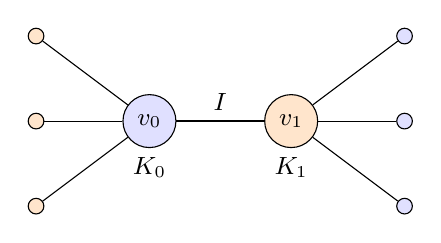
\begin{tikzpicture}[scale=.9, every node/.style={font=\small}]
\node[circle,draw,fill=blue!12] (a) at (0,0) {$v_0$};
\node[circle,draw,fill=orange!20] (b) at (2,0) {$v_1$};
\draw[thick] (a)--node[above] {$I$} (b);
\foreach \y in {-1.2,0,1.2}{
\node[circle,draw,fill=orange!20,inner sep=2pt] (l) at (-1.6,\y) {};
\draw (a)--(l);
\node[circle,draw,fill=blue!12,inner sep=2pt] (r) at (3.6,\y) {};
\draw (b)--(r);}
\node at (0,-.65) {$K_0$};
\node at (2,-.65) {$K_1$};
\end{tikzpicture}
\caption{Two adjacent vertex types and their edge stabilizer. The other branches are schematic.}
\label{fig:edge}
\end{figure}
For example, $D^m v_0$ lies at distance $|m|$ from $v_0$. The diagonal element $\operatorname{diag}(\varpi,\varpi^{-1})$ translates this apartment by two edges.

\subsection{Compact induction and characters}
For a compact open subgroup $H$ and a finite-dimensional smooth representation $\sigma$ of $H$, the compact induction $\cInd_H^G\sigma$ consists of locally constant functions $f:G\to V_\sigma$ satisfying $f(hg)=\sigma(h)f(g)$ and supported on finitely many left cosets of $H$. The action is right translation. Equivalently it is a direct sum of copies of the type space indexed by vertices when $H=K_j$. A fixed coset contributes its local trace, and a moved coset contributes zero to the diagonal trace. We justify the finite elliptic character formula in Section~\ref{sec:frob}.

A smooth representation is admissible if its invariants under every compact open subgroup are finite-dimensional. A supercuspidal representation is an irreducible admissible representation not arising as a subquotient of proper parabolic induction. For the representations under consideration, admissibility and irreducibility may be supplied by the relevant type construction. We distinguish this input from our trace comparison, which does not itself establish either property.

For example, inflate a cuspidal representation of $\mathrm{SL}_2(\mathbb F_7)$ of dimension six along $K_0\to\mathrm{SL}_2(\mathbb F_7)$, and compactly induce to $G$. This is a depth-zero construction. The resulting space is infinite-dimensional, even though the type has dimension six.

\subsection{Unramified elliptic tori}
Let $E/F$ be unramified quadratic and identify $F^2$ with $E$ using an integral basis of $\mathcal O_E$. Multiplication embeds the norm-one group $T_0=E^1$ into $K_0$. Set $T_1=DT_0D^{-1}$. These are the two rational conjugacy classes of unramified elliptic maximal tori. Indeed, conjugation by $\mathrm{GL}_2(F)$ is transitive on embeddings, and the determinant of the centralizer is the norm group, of index two with even valuation. Reduction gives the cyclic group $\bar T=\ker(N_{\mathbb F_{q^2}/\kk})$ of order $q+1$. Every element of $T_i$ except $\pm I$ is regular semisimple. For example, over $\mathbb Q_7$ we may take $E=\mathbb Q_7(\sqrt3)$, whose norm-one group consists of $\alpha+\beta\sqrt3$ with $\alpha^2-3\beta^2=1$.

\section{The double cover and local splittings}\label{sec:cover}
We retain the explicit Hilbert-symbol approach of the original notes to calculate the edge sign. This calculation is the arithmetic input for the geometric proof.

\subsection{Kubota coordinates and the two splittings}
For $g=\left(\begin{smallmatrix}a&b\\c&d\end{smallmatrix}\right)$ put $x(g)=c$ if $c\ne0$, and $x(g)=d$ otherwise. The cover has multiplication
\begin{equation}\label{eq:kubota}
 (g,\zeta)(h,\xi)=(gh,\zeta\xi\beta(g,h)),\qquad
 \beta(g,h)=\left(\frac{x(gh)}{x(g)},\frac{x(gh)}{x(h)}\right)_2.
\end{equation}
The Hilbert symbol is symmetric, bimultiplicative and trivial on pairs of units. For $a=\varpi^m u$, $b=\varpi^n v$ with units $u,v$, it is
\begin{equation}\label{eq:hilbert}
 (a,b)_2=\ell(-1)^{mn}\ell(\bar u)^n\ell(\bar v)^m.
\end{equation}
In particular $(a,-a)_2=1$. The Kubota splitting over $K_0$, cited from the standard odd-residue-characteristic construction \cite{Ku67,Ge76}, is $s_0(k)=(k,r_0(k))$, where
\begin{equation}\label{eq:r0}
 r_0(k)=
 \begin{cases}
 (c,d)_2 & cd\ne0,\ c\in\varpi\OO,\\
 1&\text{otherwise}.
 \end{cases}
\end{equation}
This is a formula on $K_0$, not a homomorphic section on all of $G$.

For example, take $k=\left(\begin{smallmatrix}1&1\\7&8\end{smallmatrix}\right)$ over $\mathbb Q_7$. Then $r_0(k)=(7,8)_2=1$. A second example over $\mathbb Q_7$ is $k=\left(\begin{smallmatrix}5&2\\7&3\end{smallmatrix}\right)$ of determinant one, for which $r_0(k)=(7,3)_2=-1$.

To transport the splitting, use the extension of the cocycle to $G'=\mathrm{GL}_2(F)$ in the original notes. Put $a(g)=\operatorname{diag}(1,\det(g)^{-1})$, $h^b=b^{-1}hb$, and
\[
 v(u,h)=
 \begin{cases}1&h_{21}\ne0,\\(u,h_{22})_2&h_{21}=0.\end{cases}
\]
The extended cocycle is
\begin{equation}\label{eq:betaext}
 \beta'(g,h)=\beta((a(g)g)^{a(h)^{-1}},a(h)h)
 v(\det h,a(g)g).
\end{equation}
We use the corresponding covering group of $G'$ and the lift $\widetilde D=(D,1)$. In particular $\widetilde D$ belongs to the larger group, not to $\Mp$. Conjugation preserves $\Mp$, and
\begin{equation}\label{eq:s1}
 s_1(k)=\widetilde D s_0(D^{-1}kD)\widetilde D^{-1}.
\end{equation}
The construction uses the standard extension in these coordinates as input. Only its diagonal specialization will be needed for the edge calculation.

\subsection{Uniqueness and equivariance}
The following elementary argument avoids exceptions in finite Schur multiplier calculations. In particular it works also for $q=3$.

\begin{lemma}\label{lem:unique}
The splittings over $K_0,K_1$ are unique. For every vertex $v$ there is a unique continuous homomorphic splitting $s_v$, and for $g\in G$ and any lift $\widetilde g$,
\[
 s_{gv}(gkg^{-1})=\widetilde g s_v(k)\widetilde g^{-1}
 \quad(k\in K_v).
\]
\end{lemma}
\begin{proof}
Two splittings differ by a continuous homomorphism $K_i\to\mu_2$. Its restriction to the pro-$p$ first congruence subgroup is trivial, because every continuous finite quotient of a pro-$p$ group is a $p$-group. It therefore factors through $\mathrm{SL}_2(\kk)$. That group is generated by the upper and lower elementary unipotent matrices, each of order $p$ or one. Their images in $\mu_2$ are trivial. Existence over the two base vertices follows from \eqref{eq:r0} and \eqref{eq:s1}. Transport by a lift of $g$ supplies existence elsewhere, and uniqueness proves independence of all choices and the asserted equivariance.
\end{proof}
For instance, over $\mathbb F_3$ the elementary unipotents have order three, so no quadratic ambiguity in the splitting arises even though this finite group is not perfect.

\subsection{The obstruction on an edge}
For the base edge let $I=K_0\cap K_1$. In the coordinates of $v_0$ it consists of integral determinant-one matrices with upper right entry in $\varpi\OO$. Its pro-$p$ radical $I^+$ is the inverse image of the lower unipotent subgroup under reduction. Thus $I/I^+\simeq\kk^\times$ via the upper left entry. This orientation is determined by our choice of $D$.

\begin{proposition}[Edge discrepancy]\label{prop:edge}
If $k=\left(\begin{smallmatrix}a&b\\c&d\end{smallmatrix}\right)\in I$, then
\begin{equation}\label{eq:edge}
 s_1(k)s_0(k)^{-1}=\ell(\bar a)\in\mu_2.
\end{equation}
For an arbitrary edge the same formula holds in transported coordinates. Reversing the orientation replaces the diagonal entry by its inverse and leaves the quadratic sign unchanged.
\end{proposition}
\begin{proof}
The ratio of two splittings is a homomorphism into the central kernel. It is trivial on $I^+$, which is pro-$p$, and is determined by its values on $h(u)=\operatorname{diag}(u,u^{-1})$ for $u\in\OO^\times$. Formula \eqref{eq:r0} gives $s_0(h(u))=(h(u),1)$. Since $D$ commutes with $h(u)$ downstairs, the ratio in \eqref{eq:s1} is the commutator of their lifts. From \eqref{eq:betaext}, using $a(D)D=h(\varpi)$, one gets
\[
 \beta'(D,h(u))=\beta(h(\varpi),h(u))=(u^{-1},\varpi^{-1})_2,
\]
whereas
\[
 \beta'(h(u),D)=\beta(h(u),h(\varpi))(\varpi,u^{-1})_2=1.
\]
The ratio is $(u,\varpi)_2=\ell(\bar u)$ by \eqref{eq:hilbert}. The entire edge set is one $G$-orbit: $K_0$ acts transitively on the lines of $\kk^2$. Equivariance in Lemma~\ref{lem:unique} proves the transported formula.
\end{proof}
In particular $s_1(-I)=\ell(-1)s_0(-I)$. Over $\mathbb Q_7$ the two lifts differ by minus one, but over $\mathbb Q_5$ they coincide at $-I$. Even over $\mathbb Q_5$ the splittings differ on diagonal units with nonsquare reduction. Thus uniqueness on vertices must not be confused with compatibility on all intersections.

\section{Geometric Frobenius character formulas}\label{sec:frob}
We replace the double-coset calculation by a sum over fixed vertices, retaining the local signs that arise in the cover.

\subsection{The weighted trace sum}
For $j=0,1$ let $\sigma_j$ be a finite-dimensional smooth representation of $K_j$. Define the genuine type by
\[
 \widetilde\sigma_j(\zeta s_j(k))=\zeta\sigma_j(k),\qquad
 \pi_j=\cInd_{K_j}^G\sigma_j,\quad
 \widetilde\pi_j=\cInd_{P^{-1}(K_j)}^{\Mp}\widetilde\sigma_j .
\]
Assume both inductions are admissible, and use their regular semisimple Harish-Chandra character functions. The existence and regularity of covering-group characters are standard harmonic-analysis input \cite{Li12}. For $v=g v_j$, define $\sigma_v(k)=\sigma_j(g^{-1}kg)$ on $K_v$, up to isomorphism. Its trace is independent of the choice of $g$.

\begin{theorem}[Weighted fixed-vertex comparison]\label{thm:weighted}
Let $t\in G$ be regular elliptic, and let $w$ be a vertex fixed by $t$. Then
\begin{align}
 \Theta_{\pi_j}(t)&=\sum_{\substack{v\in Gv_j\\tv=v}}\tr\sigma_v(t),\label{eq:ordinary}\\
 \Theta_{\widetilde\pi_j}(s_w(t))
 &=\sum_{\substack{v\in Gv_j\\tv=v}}
 c_{w,v}(t)\tr\sigma_v(t),\label{eq:weighted}
\end{align}
where $c_{w,v}(t)=s_w(t)s_v(t)^{-1}\in\mu_2$. If $w=w_0,w_1,\ldots,w_d=v$ is the unique geodesic, then
\begin{equation}\label{eq:path}
 c_{w,v}(t)=\prod_{a=1}^{d}c_{w_{a-1},w_a}(t).
\end{equation}
\end{theorem}
\begin{proof}
The regular elliptic fixed set is nonempty and finite. To see nonemptiness, identify the two-dimensional space with the quadratic field $F[t]$. The eigenvalue of $t$ is a norm-one unit, so its multiplication preserves the ring of integers of this field. The fixed subtree is connected because the unique path between fixed vertices is fixed pointwise. If it were infinite, local finiteness would produce an infinite ray (choose at every step a branch containing infinitely many fixed vertices). Such a ray determines an end of the tree, hence an $F$-line in $F^2$. For completeness, after choosing a basis at the initial vertex, the successive vertices along a ray correspond to compatible rank-one directions modulo $\varpi^m$; completeness gives a line in the inverse limit. A fixed end would give an invariant $F$-line for $t$, contrary to its irreducible characteristic polynomial.

Choose $R$ so that the fixed set lies strictly inside $B(w,R)$. There is an open neighborhood of $t$ in $K_w$ on which no vertex of the finite sphere of radius $R$ is fixed. Shrink it to make all fixed-vertex conditions inside this ball constant. By connectedness, no vertex outside the ball is fixed anywhere in this neighborhood. The same holds on its lift near $s_w(t)$.

In the compact-induction function model, an operator associated with a locally constant compactly supported test function on this neighborhood is finite rank by admissibility. Its diagonal blocks are the integrals of the local type operators over those group elements fixing the corresponding coset. Only the finitely many indicated cosets can have nonzero diagonal blocks. The trace of a finite-rank operator on an algebraic direct sum equals the sum of its diagonal block traces. Equivariance of the splittings identifies the genuine local trace with $c_{w,v}(t)\tr\sigma_v(t)$; the factor is locally constant and is obtained by writing $s_w(t)=c_{w,v}(t)s_v(t)$. Integrating proves the two distribution identities on this neighborhood. Local constancy of the regular character functions then gives the pointwise formulas. Finally the path lies in the fixed subtree, so every splitting in \eqref{eq:path} is defined at $t$. Multiplication telescopes the ratios.
\end{proof}

For example, if $t$ fixes only $v_0$, the character of a representation induced from the other vertex type vanishes, and no edge discrepancy enters the formula.

\subsection{The constant parity factor}
The characteristic polynomial of $t$ has the same reduction at every fixed vertex, because trace and determinant are independent of the lattice basis. If it fixes an edge, that reduction has roots in $\kk$, since the edge reduction is triangular.

\begin{lemma}\label{lem:repeated}
If a regular elliptic element $t$ fixes an edge, its reduced characteristic polynomial is $(X-z)^2$ for $z=\pm1$.
\end{lemma}
\begin{proof}
Distinct roots in $\kk$ would lift by Hensel's lemma to roots in $F$, contradicting ellipticity. Thus the roots coincide, and determinant one gives $z^2=1$.
\end{proof}

\begin{corollary}[Corrected direct comparison]\label{cor:compare}
Under the hypotheses of Theorem~\ref{thm:weighted}, suppose $w$ has type $i$. If the fixed set contains an edge, let $z$ be as in Lemma~\ref{lem:repeated}. Then
\begin{equation}\label{eq:parity}
 \Theta_{\widetilde\pi_j}(s_w(t))
 =\ell(z)^{j-i}\Theta_{\pi_j}(t).
\end{equation}
If the fixed set is a single vertex, the ordinary and genuine characters agree at its canonical lift for both inducing types. In particular the equality holds without a sign for any regular elliptic $t\in K_j$ at $s_j(t)$.
\end{corollary}
\begin{proof}
Each edge of the fixed subtree has triangular reduction with diagonal entries $z,z$. Proposition~\ref{prop:edge} gives the same sign $\ell(z)$ on every edge. Since $d(w,v)\equiv j-i\pmod2$, the weight in \eqref{eq:weighted} is independent of the summation vertex. The single-vertex case follows directly from the empty sum or the weight one. Taking $w=v_j$ proves the last claim.
\end{proof}
For instance, this yields an elliptic comparison for any strongly cuspidal positive-depth type of the original notes for which both compact inductions are admissible. No formula for the individual finite type traces is needed. The conclusion does not assert a classification of all positive-depth representations.

\section{Explicit unramified depth-zero formulas}\label{sec:depthzero}
We now compute the ordinary and genuine characters using the finite cuspidal character table and the geometry of the fixed ball. This gives the twofold counterpart of the odd-degree companion \cite{Jo26}.

\subsection{Fixed balls}
At $v_i$, write the regular element of $T_i$ in the multiplication model for $E^1$. If its reduction is $z=\pm1$, put $r=\val_E(t-z)\ge1$. If its reduction is noncentral, put $r=0$.

\begin{proposition}\label{prop:ball}
The fixed vertices of $t\in T_i\setminus\{\pm I\}$ form $B(v_i,r)$. At interior vertices for $r\ge1$ the reduction is $zI$; at boundary vertices it is $z$ times a nonidentity unipotent.
\end{proposition}
\begin{proof}
Transport to $i=0$. Choose an integral basis $(1,\alpha)$ of $\mathcal O_E$ with $\alpha$ having trace zero and nonsquare unit square. Write $t=a+b\alpha$. For noncentral reduction $b$ is a unit. For central reduction $a\equiv z$ and $b\equiv0$ modulo $\varpi$. Since $a^2-b^2\alpha^2=1$, $(a-z)(a+z)=b^2\alpha^2$, and $a+z$ is a unit. Hence $\val(b)=\val_E(t-z)=r$. In either case the order $\OO[t]$ is $\OO+\varpi^r\mathcal O_E$.

Scale a lattice $L$ by a power of $\varpi$ so that $\mathcal O_E L=\mathcal O_E$. Then $L\subset\mathcal O_E$ contains a unit. Stability under $t$ is equivalent to stability under $\OO[t]$ (the inverse of $t$ is its trace minus $t$). Multiplication of a unit of $L$ by $\varpi^r\mathcal O_E$ shows that stability implies $\varpi^r\mathcal O_E\subset L$. Conversely the latter inclusion implies stability under the order. By elementary divisors and the normalization, this is exactly distance at most $r$.

If $d(v_0,[L])<r$, the inclusion $\varpi^r\mathcal O_E\subset\varpi L$ gives $(t-z)L\subset\varpi L$. At a boundary vertex the reduction cannot be scalar: if it were scalar, $t$ would fix all neighboring vertices, including one outside the fixed ball. Its characteristic polynomial modulo $\varpi$ is $(X-z)^2$, so it is a scalar times nonidentity unipotent.
\end{proof}
For $F=\mathbb Q_7$ and $t=(1+7^r\sqrt3)/(1-7^r\sqrt3)$ the radius is $r$. Its trace reduction is $2$ for every $r\ge1$.

\subsection{Finite cuspidal data and counting}
Let $\theta:\bar T\to\mathbb C^\times$ be regular, meaning $\theta^2\ne1$. The finite Deligne--Lusztig cuspidal representation $\sigma_\theta$ of $\mathrm{SL}_2(\kk)$ has dimension $q-1$. We use the standard generic finite character values \cite{DL76,Bo11}:
\[
 \chi_\theta(zI)=(q-1)\theta(z),\quad
 \chi_\theta(zu)=-\theta(z),\quad
 \chi_\theta(\bar\tau)=-\theta(\bar\tau)-\theta(\bar\tau^{-1}),
\]
where $u$ is nonidentity unipotent and $\bar\tau$ is regular elliptic. Inflate $\sigma_\theta$ to each $K_j$ by reduction in its own coordinates, and use the ordinary and genuine inductions of Section~\ref{sec:frob}, denoted $\pi_{j,\theta}$ and $\widetilde\pi_{j,\theta}$. Their admissibility and depth-zero supercuspidality are inputs from the linear and covering depth-zero constructions \cite{MP94,HW09}.

There are $N_0=1$ vertices at distance zero and $N_d=(q+1)q^{d-1}$ at distance $d\ge1$. Indeed, after the first step every vertex has $q$ outgoing edges farther from the center. A vertex at distance $d$ from a type-$i$ center has type $i+d$ modulo two.

\begin{theorem}[Twofold unramified character formulas]\label{thm:depthzero}
Let $t\in T_i\setminus\{\pm I\}$ and let $\bar\tau$ denote its reduction at $v_i$.
If $r=0$, both $\Theta_{\pi_{j,\theta}}(t)$ and $\Theta_{\widetilde\pi_{j,\theta}}(s_i(t))$ equal
\[
 \begin{cases}
 -\theta(\bar\tau)-\theta(\bar\tau^{-1})&j=i,\\
 0&j\ne i.
 \end{cases}
\]
If $r\ge1$ and $\bar\tau=zI$, then
\begin{align}
 \Theta_{\pi_{j,\theta}}(t)&=\theta(z)
 \bigl((-1)^{r+1+j-i}q^r-1\bigr),\label{eq:closed}\\
 \Theta_{\widetilde\pi_{j,\theta}}(s_i(t))
 &=\ell(z)^{j-i}\theta(z)
 \bigl((-1)^{r+1+j-i}q^r-1\bigr).\label{eq:closedgen}
\end{align}
\end{theorem}
\begin{proof}
When $r=0$, Proposition~\ref{prop:ball} gives just the center vertex. The finite elliptic character value proves the assertion. For $r\ge1$ write $A_r$ for the ordinary character divided by $\theta(z)$ on the type containing the boundary and $B_r$ for the other type. At depth one they are $A_1=-(q+1)$ and $B_1=q-1$. On increasing $r$ by one, all old boundary vertices change their weight from $-1$ to $q-1$, and the new boundary has the other type. Therefore $B_{r+1}=A_r+qN_r$ and $A_{r+1}=B_r-N_{r+1}$. Induction using $N_r=(q+1)q^{r-1}$ gives $A_r=-q^r-1$ and $B_r=q^r-1$. The boundary type satisfies $j-i\equiv r\pmod2$, which gives \eqref{eq:closed}. Corollary~\ref{cor:compare} gives \eqref{eq:closedgen}.
\end{proof}
For example, at radius two the center and its second sphere have the same type, and the character on that type is $-q^2-1$ times the central character.

\subsection{Packet sums and the central sign}
The ordinary two-type sum at central reduction is $-2\theta(z)$. At noncentral reduction it is $-\theta(\bar\tau)-\theta(\bar\tau^{-1})$. This is the ordinary depth-zero packet sum, with the usual restriction interpretation from $\mathrm{GL}_2(F)$ in the generic case. We do not assert that the pair of genuine representations constitutes a Langlands packet for the double cover.

\begin{corollary}\label{cor:sum}
At central reduction $z$ the signed genuine sum is
\[
 \sum_{j=0}^1\ell(z)^{j-i}
 \Theta_{\widetilde\pi_{j,\theta}}(s_i(t))=-2\theta(z).
\]
The unweighted genuine sum equals this value when $\ell(z)=1$. When $\ell(z)=-1$, it equals $2(-1)^{r+1}\theta(z)q^r$.
\end{corollary}
\begin{proof}
Insert \eqref{eq:closedgen}; the squared sign is one. In the unweighted case with $\ell(z)=-1$, the constant terms cancel and the two terms of magnitude $q^r$ add, giving the claimed expression.
\end{proof}
The distinction also follows from the central characters. In the split fiber over $-I$, the two vertex splittings differ by $\ell(-1)$. For $q\equiv3\pmod4$, inducing with the same $\theta$ from both vertex types gives opposite genuine central characters at $s_0(-I)$. Their sum should therefore not be expected to behave like the ordinary packet sum near that lift.

\section{Worked examples over $\mathbb Q_7$ and $\mathbb Q_5$}\label{sec:examples}
The examples show that the quadratic correction is measurable even in the simplest depth-zero setting. Take $E=\mathbb Q_7(\sqrt3)$ and a character $\theta$ of order eight on $\bar T$. Then $\theta(-1)=-1$. Set
\[
 t_r=\frac{1+7^r\sqrt3}{1-7^r\sqrt3}.
\]
Multiplication by $t_r$ is norm one. Its congruence depth at $v_0$ is $r$ because $t_r-1=2\cdot7^r\sqrt3/(1-7^r\sqrt3)$ has valuation $r$. The table gives the ordinary and genuine characters for $i=0$, with the genuine values evaluated at $s_0(\pm t_r)$.

\begin{center}
\small
\begin{tabular}{cccccc}
\toprule
$t$ & $r$ & Ordinary $(j=0,1)$ & Genuine $(j=0,1)$ & Genuine sum\\
\midrule
$t_r$ &1& $(6,-8)$ & $(6,-8)$ & $-2$\\
$t_r$ &2& $(-50,48)$ & $(-50,48)$ & $-2$\\
$t_r$ &3& $(342,-344)$ & $(342,-344)$ & $-2$\\
$-t_r$ &1& $(-6,8)$ & $(-6,-8)$ & $-14$\\
$-t_r$ &2& $(50,-48)$ & $(50,48)$ & $98$\\
$-t_r$ &3& $(-342,344)$ & $(-342,-344)$ & $-686$\\
\bottomrule
\end{tabular}
\end{center}
At depth one, the center contributes six and the eight neighbors contribute minus one each near $I$. Near $-I$ the finite central character multiplies both ordinary values by minus one. The edge discrepancy introduces one further minus sign on the odd orbit. All numbers follow by exact substitution into \eqref{eq:closed} and \eqref{eq:closedgen}.

Over $\mathbb Q_5$ take $E=\mathbb Q_5(\sqrt2)$ and a character of order six. Here $\theta(-1)=-1$ but $\ell(-1)=1$. The ordinary and genuine values near $-I$ at radius one are both $(-4,6)$, and the sum is $2$. At radius two both are $(26,-24)$. Thus the difference between the two examples is not an artifact of the choice of type.

\section{Relation to the original cocycle and double-coset method}\label{sec:old}
We explain how the older approach fits the geometric proof and isolate its remaining analytic questions. The original notes use $\omega=D^{-1}$ and diagonal matrices $h(\varpi^m)$, together with the Weyl element $w_0=\left(\begin{smallmatrix}0&-1\\1&0\end{smallmatrix}\right)$. Their actions on the standard apartment are translations of even length and reflection about $v_0$, respectively. Their double cosets organize orbits of a pro-$p$ Iwahori on the vertices. With the present orientation $I^+$ consists of matrices reducing to lower unipotents. Equivalently the upper-unipotent convention corresponds to the adjacent vertex $D^{-1}v_0$ instead.

The original diagonal conjugation calculation has a useful special case: for $h(u)\in G$ and any $g\in G$, conjugating $(g,\zeta)$ by $(h(u),1)$ preserves the Kubota coordinate $\zeta$. Indeed if $c\ne0$, the three factors in the conjugation sign from \eqref{eq:kubota} are $(u,u)_2$, $(c,u^{-1})_2$ and $(u,u c)_2$. Their product is one. If $c=0$, replace $c$ by $d$ in the second factor and the third by $(u,d u)_2$, with the same result. This does not imply that the coordinates of two canonical splittings agree. For example, Proposition~\ref{prop:edge} shows the obstruction for the determinant-$\varpi$ translation, which is not an element of $G$.

On the regular elliptic domain Theorem~\ref{thm:weighted} supplies a finite termwise comparison and Corollary~\ref{cor:compare} recovers the same-inducing-type direct identity on $K_j$. On conjugates of $K_j$, the correct lift is the transported one, not an unqualified value of $r_j$ outside its domain. If a regular elliptic element fixes no vertex of type $j$, both characters vanish.

\begin{remark}[Remark 2026.1: split regular elements]\label{rem:split}
The original notes also assert a direct comparison on the split Cartan. A compact regular split element fixes an entire apartment, so the ungrouped fixed-vertex sum need not be finite or absolutely convergent. A proof requires the grouping or regularization appropriate to the compact-induction character formula, with an independent justification for the cover. Proposition~\ref{prop:edge} shows that along a fixed split apartment the edge sign is $\ell(\bar u)$ for a diagonal unit $u$. When this is $-1$, the weights alternate between vertex types, but for a sum over a single type they agree along paths within the apartment. Establishing the effect of branches away from the apartment and the analytic passage to pointwise characters remains to be done. No split character theorem is claimed here.
\end{remark}
For example, $\operatorname{diag}(3,3^{-1})$ over $\mathbb Q_7$ is regular split and fixes the standard apartment. Unlike the elliptic example, the argument excluding fixed vertices beyond a finite sphere cannot apply.

\section{Positive depth, ramified tori, and the power map}\label{sec:extensions}
The parity comparison is more general than the explicit finite-field calculation. We describe the remaining research directions without attributing new classification results to the 1996 notes.

\subsection{Positive-depth types}
For a strongly cuspidal type of level $m>1$ in the sense of Manderscheid, provided both compact inductions are admissible, Corollary~\ref{cor:compare} holds on the regular elliptic set with the same sign. It does not depend on the depth of the inducing type. For example, a type factoring through $K_0/K_0(m)$ has a finite local trace at each fixed vertex, but that trace is not generally determined by reduction modulo $\varpi$. Determining these traces in terms of the level and the element's congruence depth is a natural next calculation.

\begin{remark}[Remark 2026.2: higher levels]
The original parameters $\sigma(\lambda,m,\alpha)$ and $\sigma_0(\lambda)$ should be matched precisely with the modern type notation, including the exceptional parameters and any reducibility or intertwining conditions. The comparison theorem is conditional on admissibility of the two inductions, rather than an unverified claim that all the parameters in the notes give precisely the desired supercuspidals.
\end{remark}

\subsection{Ramified elliptic elements}
The general elliptic theorem already covers ramified tori at the level of a weighted sum. In a ramified quadratic extension a norm-one element preserves the lattice $\mathcal O_E$ and its maximal ideal, which are adjacent as $\OO$-lattices. For example, $\mathbb Q_7(\sqrt7)$ has such a pair of lattices. The fixed subtree therefore includes an edge, and the parity factor follows from Lemma~\ref{lem:repeated}. Explicit depth-zero evaluations require a separate fixed-subtree radius computation centered on this edge. We leave that calculation open rather than import the unramified formula.

\subsection{Squaring and theta correspondence}
The square map on $\bar T$ has kernel $\{\pm1\}$ and image of index two. On the full unramified norm-one torus the same obstruction remains, since squaring is an automorphism on its pro-$p$ kernel of reduction. Consequently no inverse-square exponent modulo $q+1$ exists. Over $\mathbb F_7$ the order-eight torus illustrates the obstruction: its square image has four elements. A root-sum relation would have to account for both $t$ and $-t$ and their possibly different lifted central signs. Such a relation is not established here.

The Shimura--Waldspurger correspondence relates genuine representations of the double cover to representations of $\mathrm{PGL}_2(F)$ and its inner forms. It is not identical to the direct compact-induction comparison with $\mathrm{SL}_2(F)$. The relationship between the signed formulas above and theta correspondence is a further question, for which \cite{Wa91,Ma04} provide starting points.

\section{Summary and open problems}\label{sec:summary}
The geometric formulation separates the ordinary trace weights from the central sign. Proposition~\ref{prop:edge} computes this sign on edges by a Hilbert-symbol calculation. Theorem~\ref{thm:weighted} and Corollary~\ref{cor:compare} propagate it through the fixed subtree and recover the direct elliptic comparison on the inducing compact subgroup. Theorem~\ref{thm:depthzero} evaluates the generic unramified depth-zero case explicitly, including the sign on the opposite vertex type. Corollary~\ref{cor:sum} explains why the ordinary cancellation has a signed genuine analogue. For $q=7$, the unweighted genuine sum near the lift of $-I$ can grow as $2q^r$ in magnitude, whereas the signed sum remains constant.

The main open tasks are to establish the grouped split character formula, compute ramified fixed-edge sums, work out explicit positive-depth traces, analyze exceptional quadratic finite parameters, and compare the signed formulas with the theta correspondence. These are not assumptions needed for the elliptic results proved here.

\section*{Glossary}
\addcontentsline{toc}{section}{Glossary}
The following terms provide a reference for readers from algebra or graph theory.
\begin{description}[style=nextline,leftmargin=1.5em]
\item[Admissible representation] A smooth representation with finite-dimensional invariants under compact open subgroups. This permits traces of test-function operators even on infinite-dimensional representation spaces.
\item[Apartment] A bi-infinite geodesic of the tree associated with two complementary $F$-lines. A split torus preserves such a geodesic.
\item[Ball and sphere] The ball contains all vertices at distance at most a specified radius. The sphere consists of vertices at exactly that distance and is the boundary of the ball.
\item[Borel subgroup] A maximal connected solvable algebraic subgroup, such as the upper triangular subgroup of $\mathrm{SL}_2$. Its finite analogue has a unipotent radical and a diagonal quotient.
\item[Bruhat--Tits tree] The tree of homothety classes of lattices in $F^2$. Its valency is $q+1$ because neighbors correspond to residue-field lines.
\item[Central extension] A surjective group homomorphism with central kernel. The double cover has kernel $\mu_2$.
\item[Character] For a finite-dimensional representation it is the trace of the representing matrix. For admissible $p$-adic representations one uses a distribution represented by the Harish-Chandra character function.
\item[Cocycle] A function measuring the failure of a chosen section of an extension to preserve multiplication. Its cocycle identity is equivalent to associativity of the extension law.
\item[Compact induction] Smooth induction with support compact modulo the inducing subgroup. Here it produces a direct sum of copies of a finite-dimensional type indexed by vertices.
\item[Congruence depth] For an unramified elliptic element near $zI$, the largest power of the uniformizer dividing its difference from $zI$ in the distinguished lattice. It is the fixed-ball radius, not the depth of the representation.
\item[Cuspidal finite representation] An irreducible representation with no invariants under unipotent radicals of proper rational parabolics. Such types furnish the input for depth-zero supercuspidals.
\item[Depth zero] A representation has nonzero invariants under a pro-$p$ radical of a parahoric subgroup. This does not mean that the induced representation is finite-dimensional.
\item[Edge discrepancy] The ratio of the two canonical splittings at adjacent vertices on their intersection. Here it is the quadratic residue character on the Iwahori quotient.
\item[Elliptic torus] A maximal torus anisotropic modulo the center. In $\mathrm{SL}_2(F)$ it is the norm-one group of a quadratic field extension.
\item[Fixed subtree] The vertices and edges fixed by an element. Its connectedness follows from uniqueness of geodesics.
\item[Frobenius character formula] A sum of traces over cosets fixed by the element. On the regular elliptic domain considered here the sum is finite.
\item[Genuine representation] A representation of the cover on which the nontrivial covering-kernel element acts by minus one. It cannot descend to the linear group.
\item[Geodesic] The unique shortest path between two vertices in a tree. Products of edge discrepancies telescope along it.
\item[Harish-Chandra character] The locally integrable function representing the trace distribution and locally constant on the regular semisimple set. It is not generally the trace of the action of an individual group element as an operator.
\item[Hilbert symbol] A bimultiplicative pairing of local square classes with values in $\mu_2$. In odd residue characteristic its value on a uniformizer and a unit is the quadratic residue sign.
\item[Homothety] Multiplication of a lattice by a common nonzero scalar. Identifying homothetic lattices removes scale and makes scalar matrices act trivially on the tree.
\item[Induced representation] A representation on functions transforming according to a prescribed subgroup representation. The larger group acts by translation; compact induction adds a compact-support condition modulo the subgroup.
\item[Inflation] Pullback of a quotient representation along a surjection. It preserves the representation space while enlarging the acting group.
\item[Iwahori subgroup] The stabilizer of an edge in this rank-one setting. Its pro-$p$ radical has quotient the multiplicative residue-field group.
\item[Lattice] The span of a vector-space basis over the ring of integers. Its homothety class is a vertex.
\item[Norm-one torus] The kernel of the field norm from a quadratic extension. Multiplication on that field has determinant equal to the norm, so norm-one elements embed in $\mathrm{SL}_2$.
\item[Parahoric subgroup] A compact open subgroup associated with a facet of a building. Here the vertex parahorics are $K_v$ and the edge parahorics are Iwahori subgroups.
\item[Principal series] Representations obtained by normalized induction from a Borel subgroup. In the double cover the inducing data are genuine representations of the lifted torus.
\item[Pro-$p$ group] An inverse limit of finite $p$-groups. It has no nontrivial continuous homomorphism to $\mu_2$ when $p$ is odd.
\item[Quadratic residue character] The homomorphism $\ell:\kk^\times\to\{\pm1\}$ equal to one on squares. In particular $\ell(-1)=(-1)^{(q-1)/2}$.
\item[Regular semisimple] An element with distinct eigenvalues over an algebraic closure in this rank-one group. Regular elliptic elements have irreducible characteristic polynomial over $F$.
\item[Splitting] A homomorphic right inverse of a covering projection on a subgroup. Unique vertex splittings need not agree on edge intersections.
\item[Stable packet sum] A sum of characters constant on regular elements within stable conjugacy classes. The ordinary depth-zero pair has this interpretation, unlike the unweighted genuine sum asserted nowhere in this paper.
\item[Supercuspidal representation] An irreducible admissible representation not a subquotient of induction from a proper parabolic subgroup. The types in the original notes are designed to construct such representations.
\item[Type] A compact subgroup representation used to characterize a class of smooth representations. Here it is the finite-dimensional input to compact induction.
\item[Unipotent element] A matrix whose eigenvalues are all one. Boundary reductions in the fixed-ball formula are central scalars times nonidentity unipotents.
\item[Vertex type] The parity of distance from the base vertex. The determinant-one group preserves the two types, and the determinant-$\varpi$ matrix interchanges them.
\end{description}

\section*{Acknowledgments}
\addcontentsline{toc}{section}{Acknowledgments}
The original notes were written by David Joyner following conversations with Jeff Adams and Jason Schultz in 1996. Sol-ChatGPT (OpenAI) assisted in drafting this geometric revision, identifying the edge discrepancy, developing the weighted comparison and explicit depth-zero formulas, and organizing the exposition. AI review is not an independent certification of the mathematical results. Further details on AI usage, changes of status, and citation verification are recorded in the separate revision log.

\begin{thebibliography}{HW09}
\bibitem[Bo11]{Bo11} C. Bonnaf\'e, \emph{Representations of $\mathrm{SL}_2(\mathbb F_q)$}, Springer, 2011.
\bibitem[DL76]{DL76} P. Deligne and G. Lusztig, Representations of reductive groups over finite fields, Ann. of Math. \textbf{103} (1976), 103--161.
\bibitem[Ge76]{Ge76} S. Gelbart, \emph{Weil's Representation and the Spectrum of the Metaplectic Group}, Lecture Notes in Math. 530, Springer, 1976.
\bibitem[HW09]{HW09} T. Howard and M. Weissman, Depth-zero representations of nonlinear covers of $p$-adic groups, IMRN (2009), 3979--3995.
\bibitem[Jo99]{Jo99} D. Joyner, A correspondence for the supercuspidal representations of the metaplectic cover of $\mathrm{SL}_2(F)$, $F$ $p$-adic, Arch. Math. \textbf{73} (1999), 332--340.
\bibitem[Jo26]{Jo26} D. Joyner, Argon, and ChatGPT, \emph{Two-orbit unramified elliptic character relations for depth-zero representations of metaplectic covers of $\mathrm{SL}_2$}, Draft 3, 2026, companion manuscript in the trace-formulas repository.
\bibitem[Ku67]{Ku67} T. Kubota, Topological covering of $\mathrm{SL}(2)$ over a local field, J. Math. Soc. Japan \textbf{19} (1967), 114--121.
\bibitem[Ku87]{Ku87} P. Kutzko, Character formulas for supercuspidal representations of $\mathrm{GL}(\ell)$, $\ell$ a prime, Amer. J. Math. \textbf{109} (1987), 201--222.
\bibitem[Li12]{Li12} W.-W. Li, La formule des traces pour les rev\^etements de groupes r\'eductifs connexes. II. Analyse harmonique locale, Ann. Sci. \'Ec. Norm. Sup. \textbf{45} (2012), 787--859.
\bibitem[Ma84a]{Ma84a} D. Manderscheid, On the supercuspidal representations of $\mathrm{SL}(2)$ and its two-fold cover I, Math. Ann. \textbf{266} (1984), 287--295.
\bibitem[Ma84b]{Ma84b} D. Manderscheid, On the supercuspidal representations of $\mathrm{SL}(2)$ and its two-fold cover II, Math. Ann. \textbf{266} (1984), 297--305.
\bibitem[Ma04]{Ma04} D. Manderscheid, Waldspurger's involution and types, J. London Math. Soc. \textbf{70} (2004), 567--578.
\bibitem[MP94]{MP94} A. Moy and G. Prasad, Unrefined minimal $K$-types for $p$-adic groups, Invent. Math. \textbf{116} (1994), 393--408.
\bibitem[Ne86]{Ne86} J. Neukirch, \emph{Class Field Theory}, Springer, 1986.
\bibitem[SS68]{SS68} P. Sally and J. Shalika, Characters of the discrete series of representations of $\mathrm{SL}(2)$ over a local field, Proc. Natl. Acad. Sci. USA \textbf{61} (1968), 1231--1237.
\bibitem[Wa91]{Wa91} J.-L. Waldspurger, Correspondances de Shimura et quaternions, Forum Math. \textbf{3} (1991), 219--307.
\end{thebibliography}
\end{document}
